\documentclass[12pt]{article}
\usepackage{amssymb,amsmath,graphicx,mathtools}
\usepackage{listings}
\usepackage[margin=0.75in]{geometry}
\parindent 16 pt
\usepackage{fancyhdr}
\pagestyle{fancy}
\fancyhead[R]{Swupnil Sahai}
\fancyhead[L]{Hierarchical Model}
\DeclarePairedDelimiter\ceil{\lceil}{\rceil}
\DeclarePairedDelimiter\floor{\lfloor}{\rfloor}

\lstset{
    language=R,
    basicstyle=\scriptsize\ttfamily,
    stepnumber=1,
    numbersep=5pt,
    showspaces=false,
    showstringspaces=false,
    showtabs=false,
    frame=single,
    tabsize=2,
    captionpos=b,
    breaklines=true,
    breakatwhitespace=false,
    escapeinside={},
    keywordstyle={},
    morekeywords={}
    }

\begin{document}

% CUSTOM SHORTCUTS

\def\ci{\perp\!\!\!\perp}
\def\ex{\mathbb{E}}
\def\prob{\mathbb{P}}
\def\ind{\mathbb{I}}
\def\grad{\triangledown}
\def\bigo{\mathcal{O}}

\section*{General Model Framework}
We wish to split the sky map into longitudinal bins, regressing FUV ($y_{ij}$) on i100 ($x_{ij}$) within each bin $i$. As such, this problem lends itself to a hierarchical framework in which each longitudinal bin has its own slope $\gamma_{1i}$ and intercept $\gamma_{0i}$, where all of the slopes and intercepts are drawn from common prior distributions. This can be represented graphically as\footnote{$\Sigma$ denotes the set of hyper priors for $\sigma$. Currently I am using a non informative prior for $\sigma_i$.}:\\

\indent\indent\indent\indent\indent\indent\indent\indent 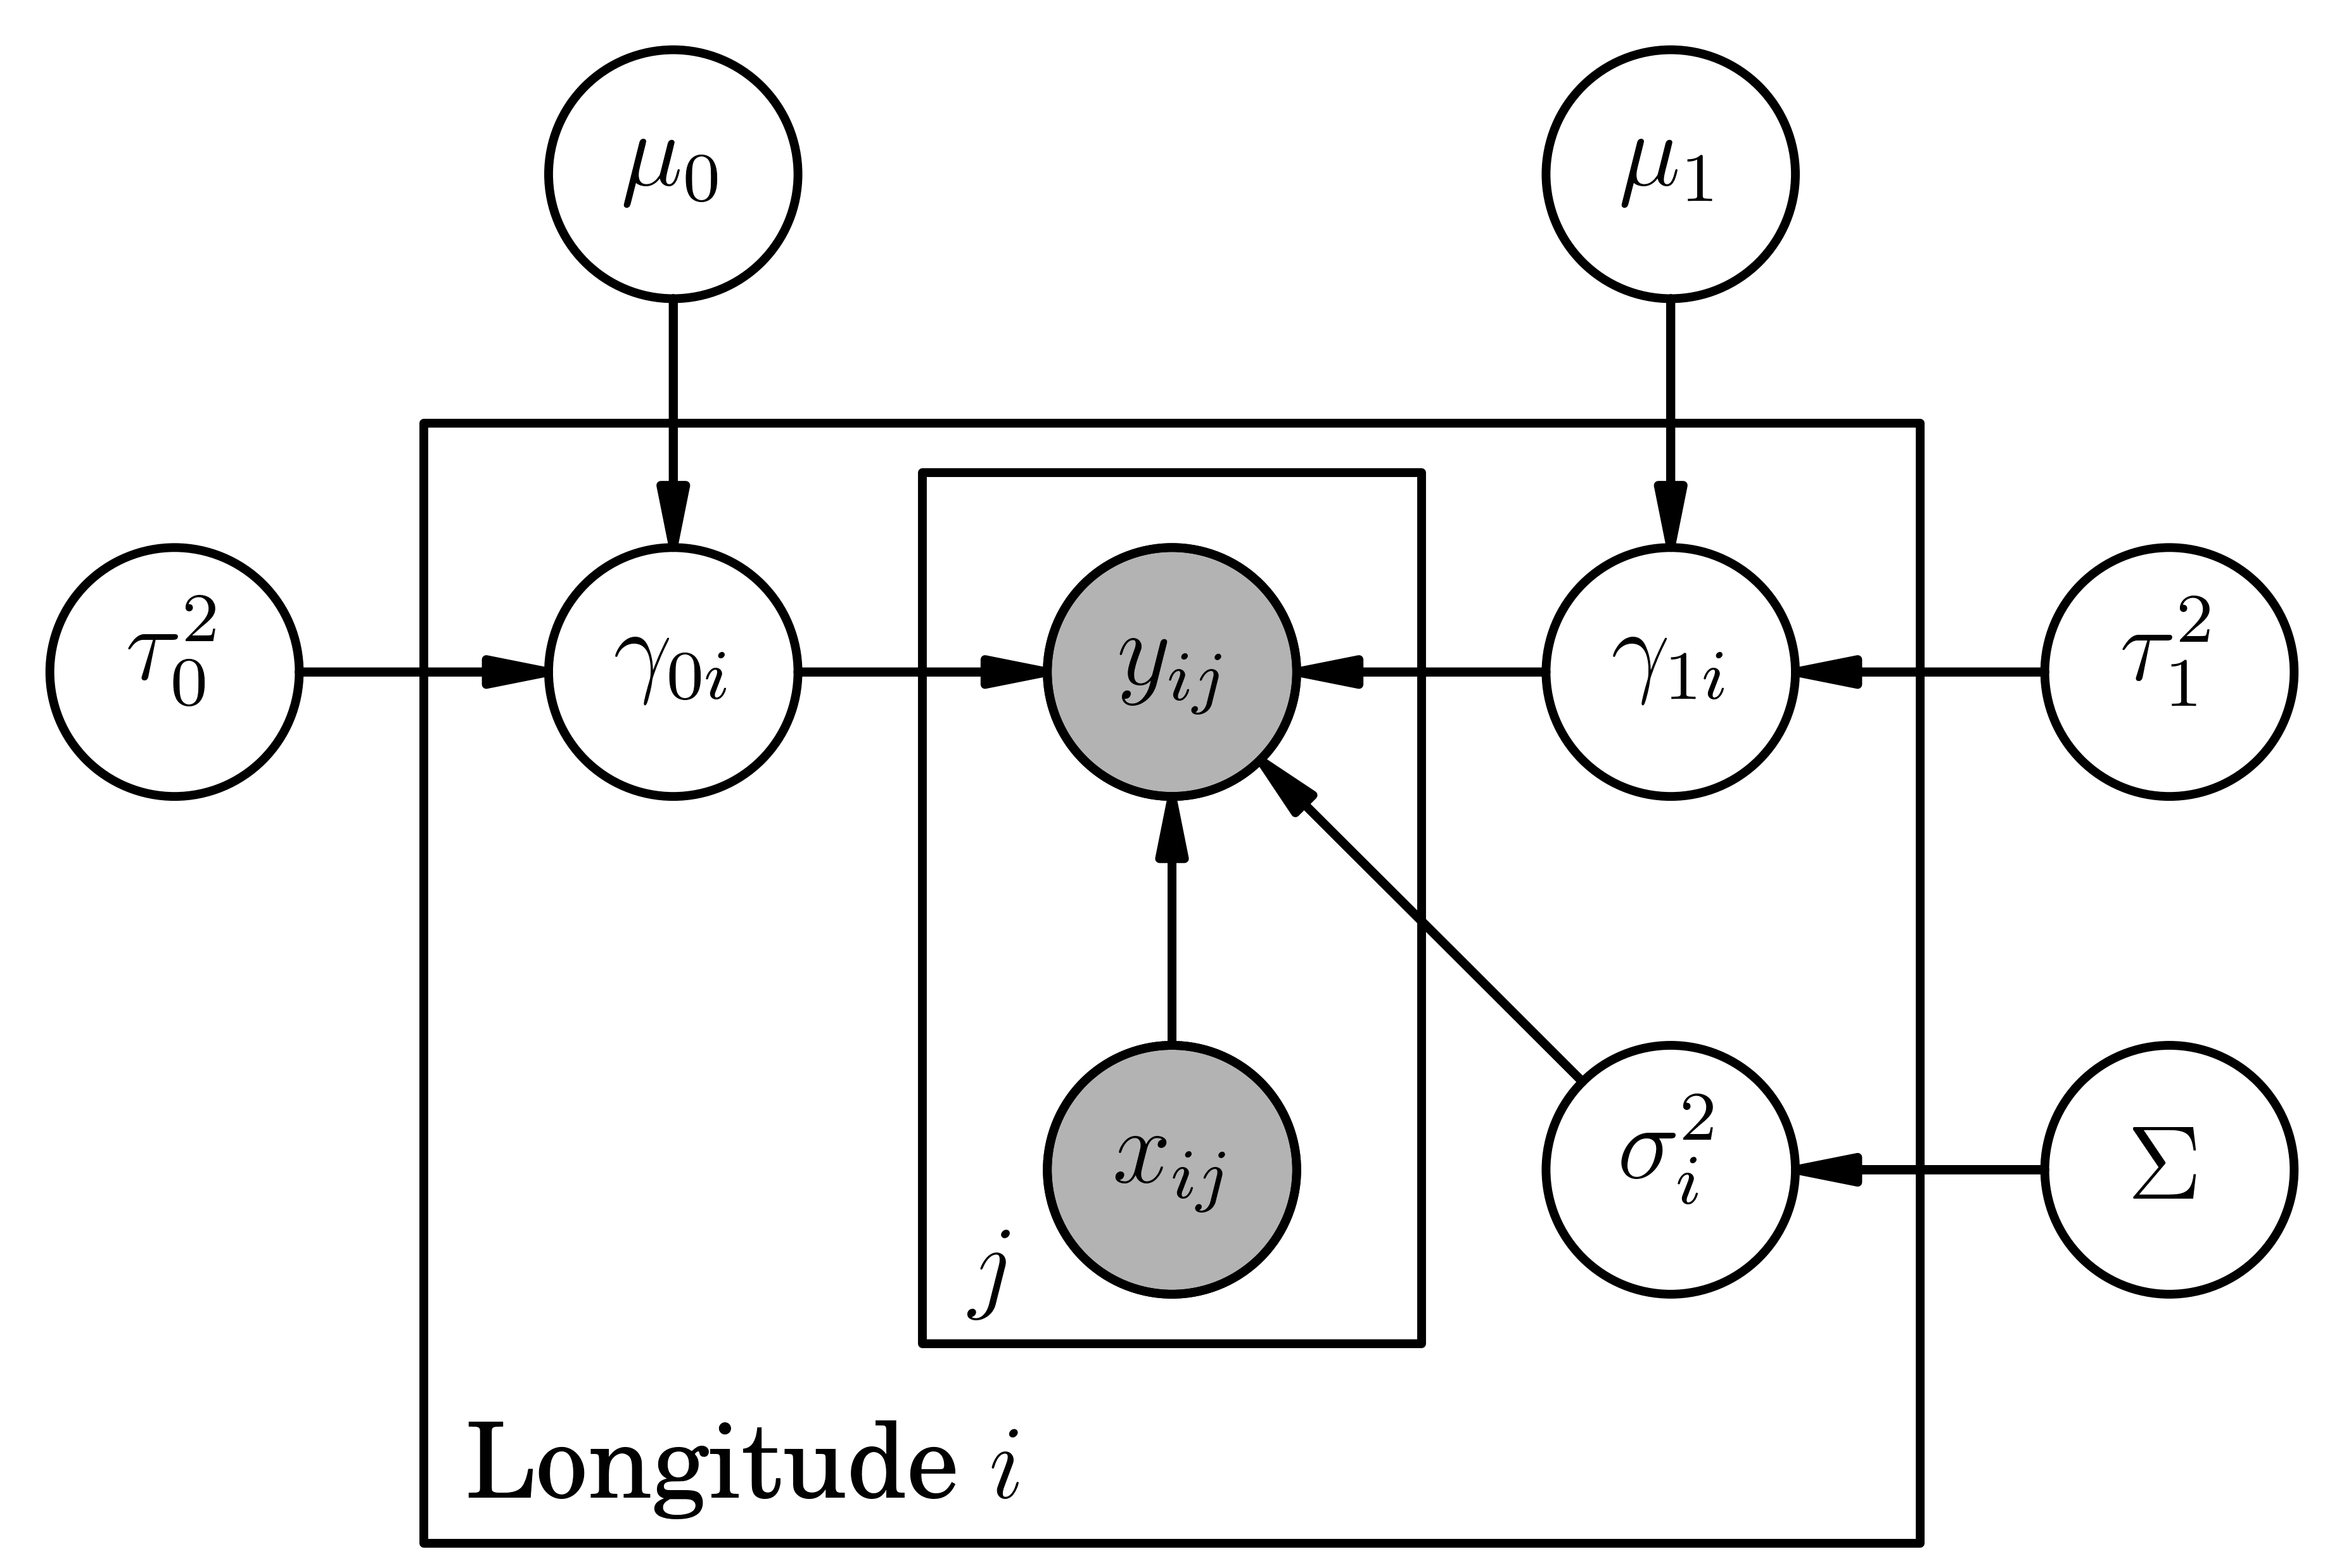
\includegraphics{Linear_Model.png}

\subsection*{Linear Model}
We initially explored $y_{ij}$ as a linear function of the parameters, so we begin with the following setup:
$$y_{ij} \sim N( \gamma_{0i} + \gamma_{1i}x_{ij} , \sigma_i^2)
\hspace{20 pt} \gamma_{0i} \sim N(\mu_0,\tau_0^2)
\hspace{20 pt} \gamma_{1i} \sim N(\mu_1,\tau_1^2)
\hspace{20 pt} \sigma_i \sim p(\sigma_i|\Sigma)$$

\subsection*{Square Root Model}
More recently, Alvin and David explored $y_{ij}$ as a square root function of the strictly positive parameters with the following setup:
$$y_{ij} \sim N( \sqrt{ \gamma_{0i}^2 + \gamma_{1i}^2 x_{ij}} , \sigma_i^2)
\hspace{20 pt} \gamma_{0i} \sim N(\mu_0,\tau_0^2)
\hspace{20 pt} \gamma_{1i} \sim N(\mu_1,\tau_1^2)
\hspace{20 pt} \sigma_i \sim p(\sigma_i|\Sigma)$$

\pagebreak
\section*{Linear Model Fitting}
I fit the hierarchical linear model in Stan using 36 longitudinal bins and sampling 100 data points from each bin, with 4 chains of 1000 iterations (Total Run Time: 2.5 Minutes).  The posterior means of all of the parameters are shown below:

\indent\indent 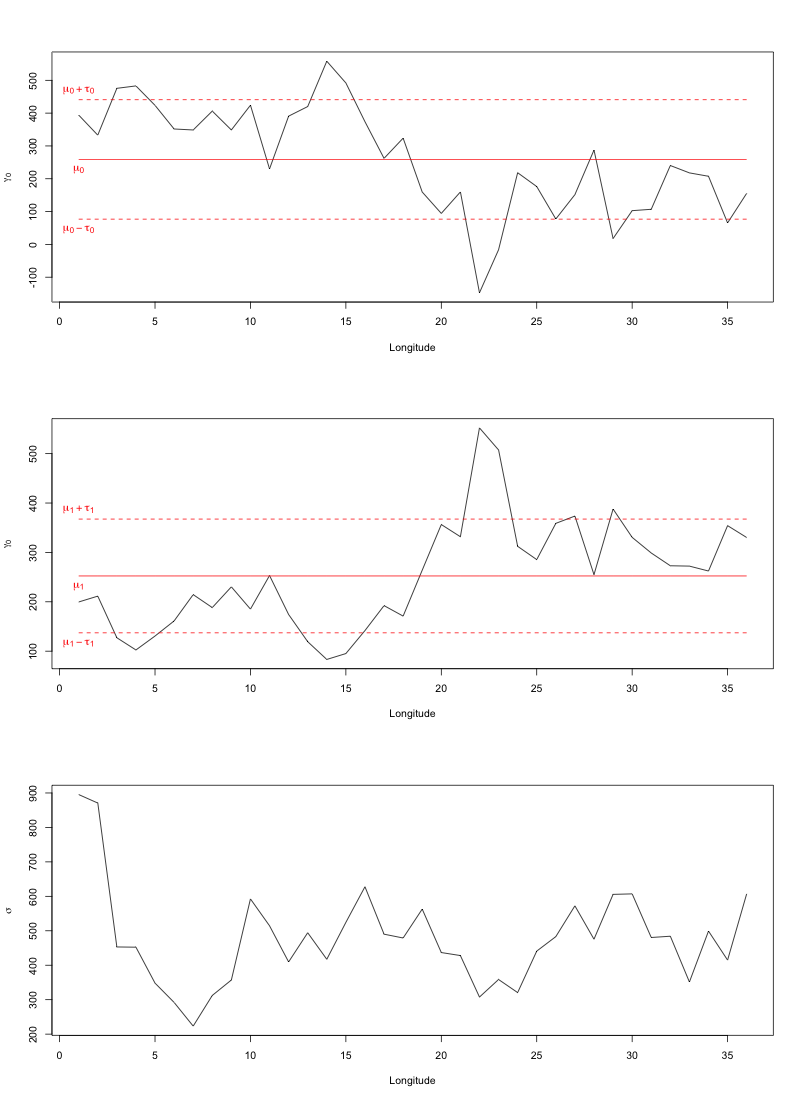
\includegraphics[scale=0.55]{params.png}

\pagebreak
\section*{Square-Root Model Fitting}
I then fit the hierarchical square-root model in Stan using 36 longitudinal bins and sampling 100 data points from each bin, with 4 chains of 1000 iterations (Total Run Time: 5 Minutes).  The posterior means of all of the parameters are shown below:

\indent\indent 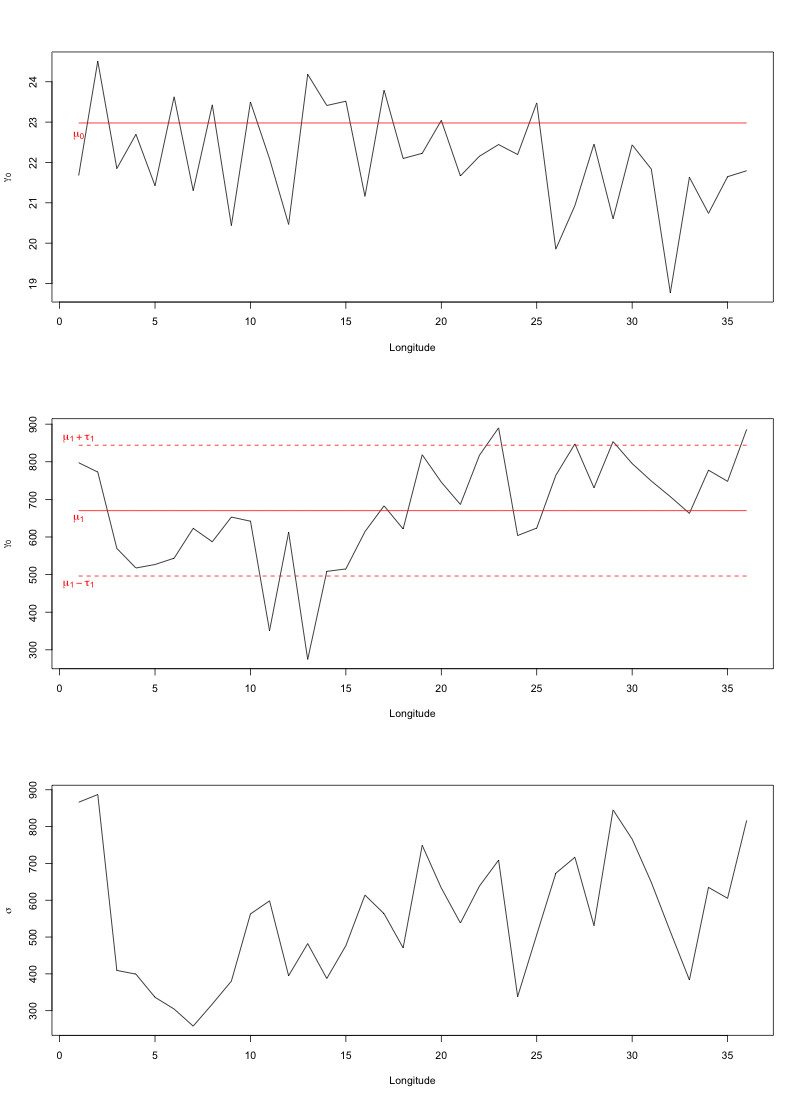
\includegraphics[scale=0.55]{params2.png}

\pagebreak
\section*{Gamma Hyperprior}
Another way to make strictly positive parameters would be to try the following setup:
$$y_{ij} \sim N( \gamma_{0i} + \gamma_{1i}x_{ij}, \sigma_i^2)
\hspace{20 pt} \gamma_{0i} \sim \text{Gamma}(\alpha_0,\beta_0)
\hspace{20 pt} \gamma_{1i} \sim \text{Gamma}(\alpha_1,\beta_1)
\hspace{20 pt} \sigma_i \sim p(\sigma_i|\Sigma)$$
which would be represented graphically as:\\ \\
\indent\indent\indent\indent\indent\indent\indent\indent 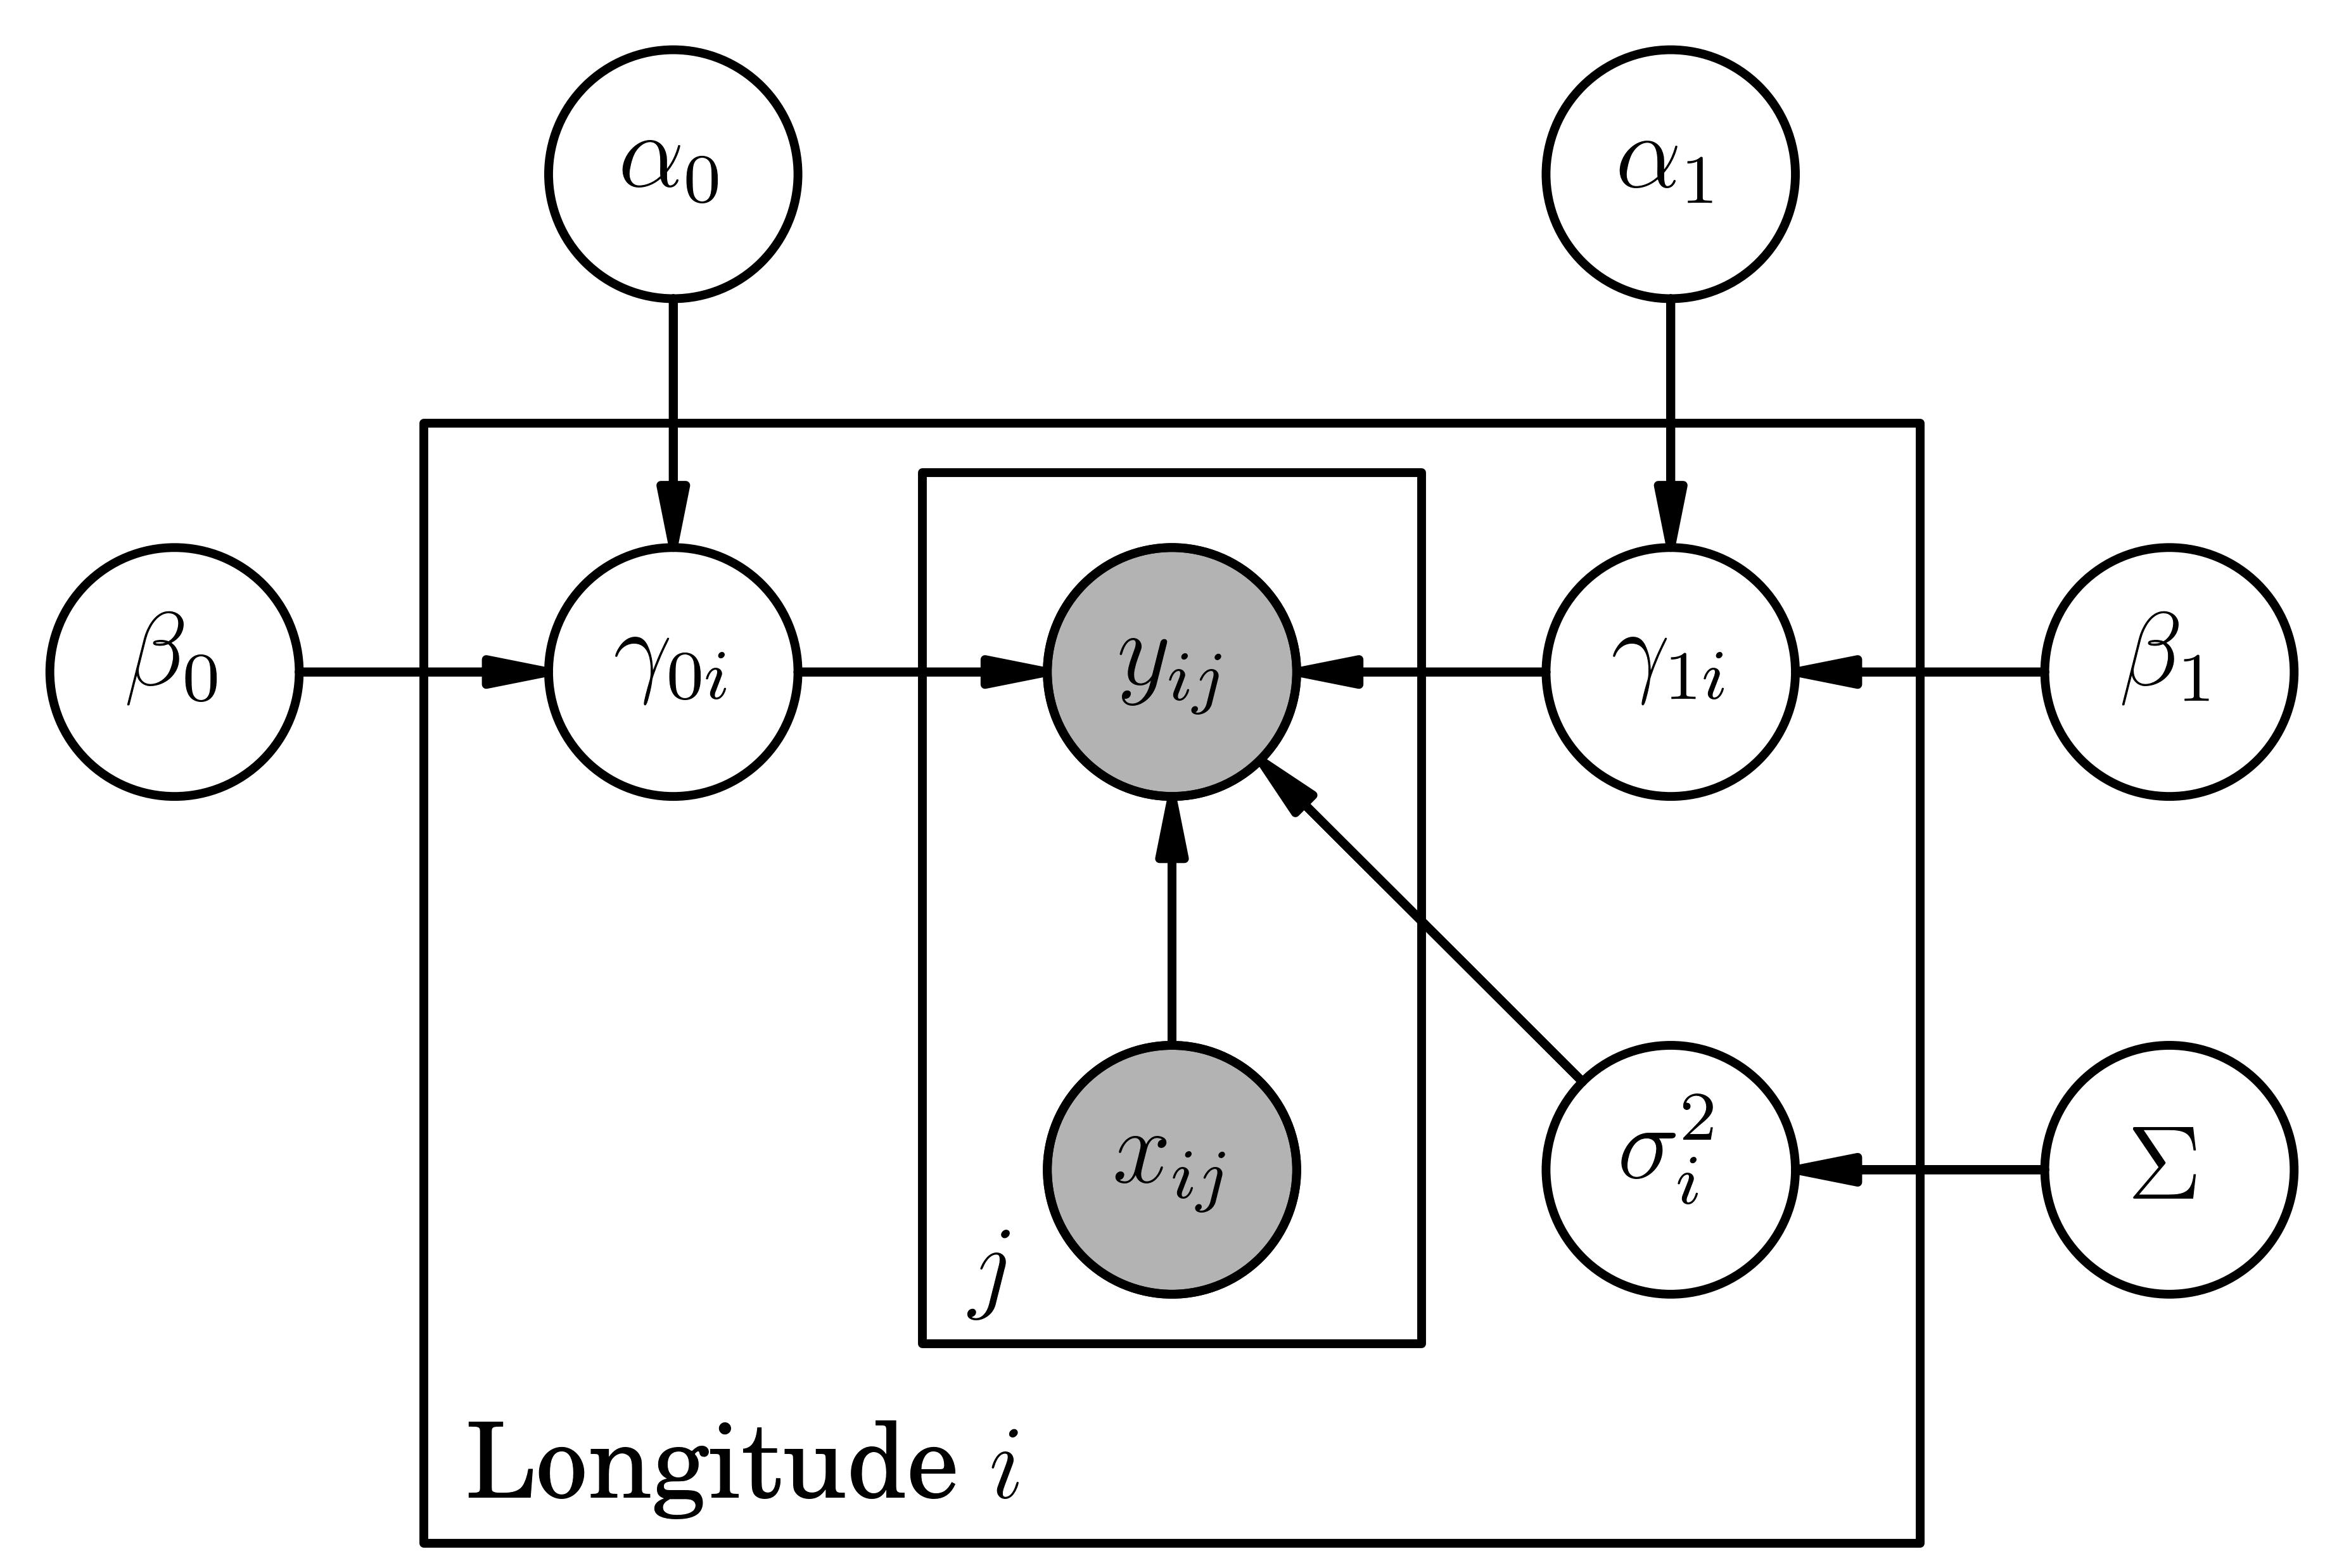
\includegraphics{SquareRoot_Model.png}\\ \\
I tried fitting this model in Stan but had several issues with the initial values. For some reason, the gamma hyper prior prevented Stan from being able to find initialization points, timing out after 100 attempts to do so. The same error was encountered even when I restricted the support of $\alpha$ and $\beta$.

%CODE
%\pagebreak
%\section{Code}
%\texttt{\lstinputlisting{hierarchical_model.R}}

\end{document}